\documentclass[letterpaper, 12pt]{article}
\usepackage{graphicx} % Required for inserting images
\usepackage{textcomp}
\usepackage{fullpage}
\usepackage{amsmath}
\usepackage{xcolor}
\usepackage{float}
\usepackage{geometry}
\geometry{margin=1in}
\usepackage{enumitem}
\usepackage{hyperref}
\usepackage{microtype}
\usepackage{gensymb}
\usepackage{parskip}
\usepackage{tikz}
\usepackage{pgfplots}
\pgfplotsset{compat=1.18}
\usepackage{nicefrac}
\hypersetup{
    colorlinks=true,        % Enable colored links
    linkcolor=teal,         % Set color for internal links
    citecolor=teal,         % Set color for citations
    filecolor=teal,         % Set color for file links
    urlcolor=teal           % Set color for URLs
}

\title{Precalculus Honors Spring Final Study Guide}
\date{Test date: June 2, 2025}

\begin{document}

\maketitle

\section*{Notation}
\begin{enumerate}
\item Always keep writing the full limit (with ``lim'') until there are no more variables in the equation. For example:
$$\lim_{x \to 3} \frac{x^2-9}{x-3} = \lim_{x \to 3} \frac{(x+3)(x-3)}{x-3}$$
\textbf{not}:
$$\lim_{x \to 3} \frac{x^2-9}{x-3} =\frac{(x+3)(x-3)}{x-3}$$
\item When using LHR, show your justification in some way and invoke LHR before solving the problem. For example:
$$\lim_{x \to 0}{\sin x} = 0 = \lim_{x \to 0}{x}$$
$$\mathrm{LHR}$$
\textbf{do NOT write this:}
$$\lim_{x \to 0} \frac{\sin x}{x} = \frac{0}{0}$$
because $\frac{0}{0}$ does not exist.
\item Justifications should be complete and concise. For example, ``A local maximum occurs at $(a, b)$ because the first derivative changes sign from positive to negative at $x = a$.'' Don't write more than necessary!
\item Don't simplify using algebraic methods unless the question specifies otherwise to avoid losing points for algebra mistakes. Once the calculus is over, the problem is done.
\end{enumerate}

\section*{Limits and continuity}

\subsection*{Definition and applications of the limit}

\begin{itemize}

\item A \textbf{limit} is a y-value where you expect to be at a certain x-value. It does not have to equal the actual value of the function at that point.

\item If the limit from the right $\displaystyle\lim_{x \to a^+} f(x)$ equals the limit from the left $\displaystyle\lim_{x \to a^-} f(x)$, the limit exists. 

\item If the limit from the right does not equal the limit from the left, or both limits go toward negative or positive infinity, the limit does not exist (DNE).

\end{itemize}

\subsection*{Methods to evaluate limits}

\subsubsection*{Plugging in directly}
Example: Evaluate $\displaystyle\lim_{x \to 5} \frac{x^2+2}{x-2}$.


$$ \lim_{x \to 5} \frac{x^2+2}{x-2} = \frac{5^2+2}{5-2} $$
$$ = \frac{25+2}{5-2} $$
$$ = \boxed{\frac{27}{3}} $$

\subsubsection*{Algebraic methods}
Example: Evaluate $\displaystyle\lim_{x \to 3} \frac{x^2-9}{x-3}$.

Factor:

$$\lim_{x \to 3} \frac{x^2-9}{x-3}$$
$$ = \lim_{x \to 3} \frac{(x+3)(x-3)}{x-3}$$
$$ = \lim_{x \to 3} x+3$$
$$ = \boxed{6}$$

\subsubsection*{Multiplying by the conjugate}
Example: Evaluate $\displaystyle \lim_{x \to 4} \frac{\sqrt{x} - 2}{x - 4} $.

Multiply the numerator and denominator by the conjugate of the numerator:

$$  \lim_{x \to 4} \frac{\sqrt{x} - 2}{x - 4} = \lim_{x \to 4} \frac{\sqrt{x} - 2}{x - 4} \cdot \frac{\sqrt{x} + 2}{\sqrt{x} + 2} $$
$$ = \lim_{x \to 4} \frac{(\sqrt{x} - 2)(\sqrt{x} + 2)}{(x - 4)(\sqrt{x} + 2)} $$  
$$ = \lim_{x \to 4} \frac{x - 4}{(x - 4)(\sqrt{x} + 2)} $$
$$ = \lim_{x \to 4} \frac{1}{\sqrt{x} + 2} $$
$$ = \frac{1}{\sqrt{4} + 2} $$  
$$ = \frac{1}{2 + 2} $$  
$$ = \boxed{\frac{1}{4}} $$


\subsubsection*{L'Hôpital's rule for indeterminate forms}
(when the limit = $\frac{0}{0}$ or $\frac{\infty}{\infty}$)

Example: Evaluate $\displaystyle \lim_{x \to 0} \frac{\sin x}{x} $.

This is an indeterminate form ($\frac{0}{0}$), requiring the application of L'Hôpital's rule (LHR). \textbf{Before anything, invoke LHR and justify. This step is very important and should not be skipped over.}

$$\lim_{x \to 0}{\sin x} = 0 = \lim_{x \to 0}{x}$$
$$\mathrm{LHR}$$

Apply L'Hôpital's rule, taking the derivative of the numerator over the derivative of the denominator.\footnote{This can be applied as many times as necessary.}

$$ \lim_{x \to 0} \frac{\frac{d}{dx}(\sin x)}{\frac{d}{dx}(x)}$$  
$$ = \lim_{x \to 0} \frac{\cos x}{1} $$
$$ = \cos 0$$
$$ = \boxed{1} $$

\section*{The derivative and its applications}

\subsection*{Definitions of the derivative}

\subsubsection*{Conceptual}
The \textbf{derivative} is the slope of a function at a given point or over the entire curve (instantaneous rate of change, IROC).

\subsubsection*{Limit definition}

$$f(x) = \lim_{h \to 0} \frac{f(x+h)-f(x)}{h}$$

\subsubsection*{Alternate limit definition}
for finding the limit at a given point $a$:

$$f'(a) = \lim_{x \to a} \frac{f(x)-f(a)}{x-a}$$

\subsection*{Basic derivatives}

$c$ denotes a constant. Differentiation is with respect to $x$.

\subsubsection*{Power rule}
$$\frac{d}{dx} x^c = cx^{c-1}$$

\subsubsection*{Product rule}
$$\frac{d}{dx}  f(x) \times g(x) = f'(x)g(x) + f(x)g'(x)$$

\subsubsection*{Quotient rule}
$$\frac{d}{dx}  \frac{f(x)}{g(x)} = \frac{g(x)f'(x) - f(x)g'(x)}{(g(x))^2}$$

\subsubsection*{Chain rule}
$$\frac{d}{dx}  f(g(x)) = f'(g(x)) \cdot g'(x)$$

\subsubsection*{Logs and exponentials}
$$\frac{d}{dx}  \ln x= \frac{1}{x}$$
$$\frac{d}{dx}  \log_a x= \frac{1}{x \ln a}$$
$$\frac{d}{dx}  a^x= a^x \ln a$$
$$\frac{d}{dx}  e^x= e^x$$

\subsubsection*{Trigonometric functions}
$$\frac{d}{dx}  \sin x= \cos x$$
$$\frac{d}{dx}  \cos x= -\sin x$$
$$\frac{d}{dx}  \tan x= \sec^2 x$$
$$\frac{d}{dx}  \csc x= -\csc x \cot x$$
$$\frac{d}{dx}  \sec x= \sec x \tan x$$
$$\frac{d}{dx}  \cot x= -\csc^2 x$$
$$\frac{d}{dx}  \arcsin x= \frac{1}{\sqrt{1-x^2}}$$
$$\frac{d}{dx}  \arccos x= -\frac{1}{\sqrt{1-x^2}}$$
$$\frac{d}{dx}  \arctan x= \frac{1}{1+x^2}$$

\subsection*{Composite and inverse differentiation}

\subsubsection*{Chain rule}
\begin{quote}
``Differentiate the mother, keep the baby inside, differentiate the baby.''
\end{quote}

Example: Differentiate $(5x+3)^3$ with respect to $x$.

$$\frac{d}{dx}(5x+3)^3 = 3(5x+3)^2 \cdot 5$$
$$ = \boxed{15(5x+3)^2}$$

\subsubsection*{Common derivatives of functions}
$u$ denotes a function.

$$\frac{d}{dx}  \ln u= \frac{u'}{u}$$
$$\frac{d}{dx}  \log_a u= \frac{u'}{u \ln a}$$
$$\frac{d}{dx}  \arcsin u= \frac{u'}{\sqrt{1-u^2}}$$
$$\frac{d}{dx}  \arccos u= -\frac{u'}{\sqrt{1-u^2}}$$
$$\frac{d}{dx}  \arctan u= \frac{u'}{1+u^2}$$
$$\frac{d}{dx}  a^u= u'a^u \ln a$$
$$\frac{d}{dx}  e^u= u'e^u$$

\subsubsection*{Inverse differentiation}
A function $f(x)$ has the inverse $g(x)$. At $(a, b)$, the derivative $f'(a)$ is equal to $\displaystyle\frac{1}{g'(b)}$.

\subsection*{Linear approximation}
Use a derivative to approximate a function at a given point.

Example: Estimate $f(1.5)$ for $f(x) = \cos x$. ($\frac{\pi}{2} \approx 1.57$ for this problem.)

Find the first derivative:

$$f'(x) \cos x = - \sin x$$

Approximate at the first derivative:

$$f'\left(\frac{\pi}{2}\right) = - \sin \frac{\pi}{2} = -1 $$

This is the slope of the tangent line. Find the value of the function at $\displaystyle \frac{\pi}{2}$:

$$f\left(\frac{\pi}{2}\right) = \cos \frac{\pi}{2} = 0$$

Write the line in slope-intercept form:

$$ y - 0 = -\left(x- \frac{\pi}{2}\right) $$

Approximate $f(1.5)$ using this line, $f'(1.57)$:

$$y = -(1.5 - 1.57)$$
$$ y = -1.5 + 1.57 $$
$$ y = 0.07 $$
$$ \boxed{f(1.5) \approx 0.07} $$

\subsection*{IVT and MVT}

\subsubsection*{Intermediate Value Theorem}

If $f$ is continuous on $[a, b]$ and $k$ is any number between $f(a)$ and $f(b)$, inclusive, then there is at least one number $c$ in the interval $[a, b]$ such that $f(c) = k$.

In other words, if a function is continuous over an interval, it has a y-value for every x-value in that interval.

Example: Let $f(x) = x^3-4x+1$. Show that there is at least one root ($f(x) = 0$) in the interval $[1, 2]$.

MVT applies because this is a polynomial function and $f(x)$ is continuous over the entire interval.

\subsubsection*{Mean Value Theorem}

If $f(x)$ is continuous on $[a, b]$ and is differentiable on $(a, b)$,  then $c$ exists such that

$$f'(c) = \frac{f(b)-f(a)}{b-a}$$.

If $f(x)$ is continuous on the closed interval and differentiable on the open interval, there is a point where AROC (average rate of change, the secant line) = IROC (instantaneous rate of change, the tangent line). 

\subsection*{Graph analysis}

\subsubsection*{Extrema}
\textbf{Local (relative) extrema} can only occur within the given interval. \textbf{Absolute extrema} (the single lowest/highest point on the interval) can occur at endpoints or within the interval. 

\subsubsection*{The first derivative}
The first derivative ($y'$, $f'(x)$, $\displaystyle\frac{dy}{dx}$) determines whether a graph is \textbf{increasing or decreasing}. When the first derivative $>$0, the graph is increasing. When the first derivative $<$0, the graph is decreasing. At $\displaystyle\frac{dy}{dx}$ = 0, there is a minimum or a maximum.

\subsubsection*{The second derivative}
The second derivative ($y''$, $f''(x)$, $\displaystyle\frac{d^2y}{dx^2}$) determines the \textbf{concavity} of a graph (concave up, concave down). When the second derivative $>$0, the graph is concave up. When the second derivative $<$0, the graph is concave down. At $\displaystyle\frac{d^2y}{dx^2}$ = 0, there is a point of inflection where the graph changes concavity.

Example: Analyze the function 
$\displaystyle f(x) = x^3-3x^2+4$.
Find the interval(s) on which the function is increasing/decreasing, local extrema, interval(s) on which the function is concave up/down, and point(s) of inflection. Justify.

First derivative:

$$3x^2 - 6x$$

Set to 0:

$$ 3x^2-6x = 0$$
$$ 3x(x-2) = 0$$
$$ x = 0, x = 2$$

0 and 2 are the critical numbers. Test numbers in the following intervals by plugging them into the first derivative.

\begin{center}
\begin{tikzpicture}[scale=1.5]
  % Draw the number line
  \draw[thick, <->] (-1,0) -- (3,0) node[right] {$f(x)$};

  % Draw ticks and labels for critical points
  \foreach \x in {0,2} {
    \draw[thick] (\x,0.1) -- (\x,-0.1);
    \node[below] at (\x,-0.1) {\small $\x$};
  }

  % Label intervals with signs of f'(x)
  % Let's say: f'(x) is positive on (-∞,0), negative on (0,2), positive on (2, ∞)
  \node[above] at (-0.5,0.2) {$+$};
  \node[above] at (1,0.2) {$-$};
  \node[above] at (2.5,0.2) {$+$};

\end{tikzpicture}
\end{center}

Second derivative:

$$6x - 6 = 0$$
$$ x = 1$$

Do the same with $x<1$ and $x>1$:

\begin{center}
\begin{tikzpicture}[scale=1.5]
  % Draw the number line
  \draw[thick, <->] (0,0) -- (2,0) node[right] {$f''(x)$};

  % Draw tick and label for critical point at 1
  \draw[thick] (1,0.1) -- (1,-0.1);
  \node[below] at (1,-0.1) {\small $1$};

  % Label intervals with signs of f'(x)
  % Example: f'(x) positive on (0,1), negative on (1,2)
  \node[above] at (0.5,0.2) {$-$};
  \node[above] at (1.5,0.2) {$+$};
\end{tikzpicture}
\end{center}

Graph:

\begin{center}
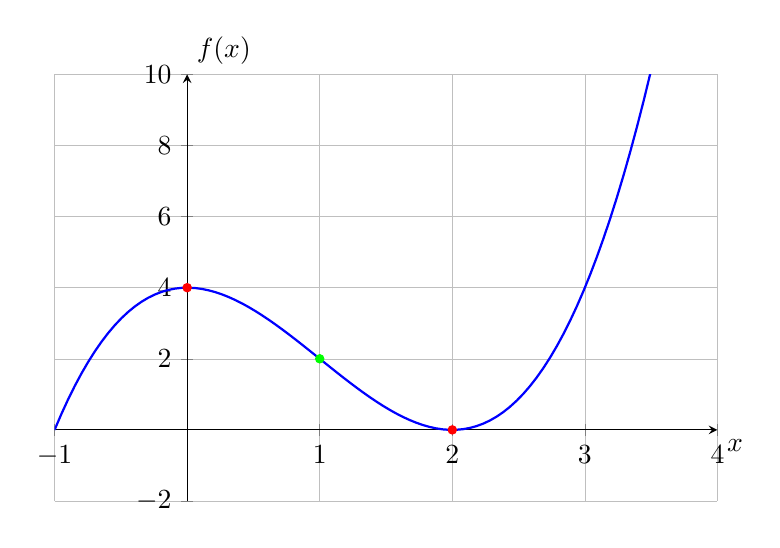
\begin{tikzpicture}
  \begin{axis}[
    axis lines = middle,
    xlabel = $x$,
    ylabel = {$f(x)$},
    domain=-1:4,
    samples=100,
    width=10cm,
    height=7cm,
    grid=both,
    grid style={line width=.1pt, draw=gray!10},
    major grid style={line width=.2pt,draw=gray!50},
    ymin=-2, ymax=10,
    xmin=-1, xmax=4,
    every axis x label/.style={at={(ticklabel* cs:1)},anchor=north west},
    every axis y label/.style={at={(ticklabel* cs:1)},anchor=south west},
 ] 
    \addplot [blue, thick] {x^3 - 3*x^2 + 4};
    % Mark critical points
    \addplot[only marks, mark=*, mark size=1.5pt, red] coordinates {(0,4) (2,0)};
    % Mark inflection point
    \addplot[only marks, mark=*, mark size=1.5pt, green] coordinates {(1,2)};
  \end{axis}
\end{tikzpicture}
\end{center}

\noindent
\framebox{%
  \begin{minipage}{\textwidth}
   \textbf{increasing}: $(-\infty, 0)$ and $(2, \infty)$ \\
   \textbf{decreasing}: $(0, 2)$ \\
   \textbf{concave up}: $(1, \infty)$ \\
   \textbf{concave down}: $(-\infty, 1)$ \\
   \textbf{maximum}: $x = 0$ because the sign of the first derivative changes from positive to negative at $x = 0$ \\
   \textbf{minimum}: $x = 2$ because the sign of the first derivative changes from negative to positive at $x = 2$ \\
   \textbf{point of inflection}: $x = 1$ because the sign of the second derivative changes from negative to positive at $x = 1$
  \end{minipage}%
}


\subsection*{Implicit differentiation}

Example 1: Find $\displaystyle\frac{dy}{dx}$ for $x^2+3xy+y=5$.

$$\frac{dy}{dx} (x^2+3xy+y) = \frac{dy}{dx} 5$$
$$ 2x + 3(xy' + y) + y' = 0$$
$$ 2x + 3xy' + 3y + y' = 0$$
$$ 3xy' + y' = -3y - 2x$$
$$ y'(3x + 1) = -3y -2x$$
$$ y' = \frac{-3y-2x}{3x+1} $$

\subsection*{Position, acceleration, and velocity}

\begin{description}
\item[position] where the object is
\item[distance] total length of path travelled 
\item[displacement] change in position from starting point to end point 
\item[velocity] the rate at which the position is changing
\item[speed] the absolute value of velocity
\item[acceleration] the rate at which the velocity is changing
\end{description}

\begin{table}[H]
\centering
\begin{tabular}{|c|c|c|}
\hline
\textbf{Original function} & \textbf{First derivative} & \textbf{Second derivative} \\\hline
position $s(t)$ & velocity $v(t)$ & acceleration $a(t)$ \\\hline
velocity $v(t)$ & acceleration $a(t)$ & - \\\hline
acceleration $a(t)$ & - & - \\
\hline
\end{tabular}
\end{table}

Example: A particle moves along a straight line with velocity given by

$$v(t) = 3t^2-12t+9$$

and position given by 

$$s(t) = t^3-6t^2+9t$$

for $t \in [0, 4]$. What is the total distance traveled and the displacement?

Find the critical numbers where the velocity is 0:

$$3t^2-12t+9 = 0$$
$$3(t^2-4t+3) = 0$$
$$(t-3)(t-1) = 0$$
$$t = 3, 1$$

The number line is separated into three intervals: from 0 to 1, 1 to 3, and 3 to 4. Test values for each interval and decide whether the object moves forward or backward depending on the sign.

When $t$ is on the interval $[0, 1]$, the object moves forward. On the interval $[1, 3]$, the object moves backward, and forward again on $[3, 4]$.

Evaluate position at both endpoints and key values:

$$s(0) = 0$$
$$s(1) = 4$$
$$s(3) = 0$$
$$s(4) = 4$$

Calculate distance between position changes.

From 0 to 1, the object moves right 4 units.

From 1 to 3, the object moves left 4 units. 

From 3 to 4, the object moves right 4 units.

$$4+4+4 = 12$$

Distance: \fbox{12 units} \\
Displacement $s(4) - s(0)$: \fbox{4 units}

\subsection*{Related rates}
For related rates problems, write the given, what you're trying to find, and a unifying equation.

Example: A balloon is being inflated so that it remains a perfect sphere. If the radius of the balloon is decreasing at a rate of 2 cm/s, how fast is the volume of the balloon decreasing when the radius is 5 cm?

Equation: $ \displaystyle V = \frac{4}{3} \pi r^3 $ \\
Given: $ \displaystyle \frac{dr}{dt} = -2$, $r = 5$ \\
Find: $\displaystyle \frac{dV}{dt}$

$$ V = \frac{4}{3} \pi r^3 $$
$$ \frac{dV}{dt} = 4 \pi r^2 \frac{dr}{dt}$$
$$ \frac{dV}{dt} = 4 \pi (5)^2 (-2)$$
$$ \frac{dV}{dt} = -200 \pi$$

The volume is \fbox{decreasing at a rate of $200 \pi \: \mathrm{cm}^3 / \mathrm{s}$} when $r = 5$.

\subsection*{Optimization}
Example: A company wants to build a rectangular fenced-in area next to a straight river, and they do not need to fence the side along the river. They have 600 meters of fencing available. What is the maximum area that can be enclosed?

Let the side across from the river be $x$, and the sides adjacent to the river be $y$. Then the perimeter of the area is

$$ 600 = x + 2y$$

This is the restriction. The area is

$$ A = xy $$

First, solve for x:

$$ x = 600 - 2y $$

plug it into the area formula:

$$ A = (600-2y)(y) $$
$$ A = 600y - 2y^2$$

To find the maximum of this equation, find the first derivative:

$$A' = 600 - 4y$$

set to 0 to find critical numbers:

$$ 0 = 600 - 4y$$
$$ -4y = -600 $$
$$ y = 150 $$

going back to the original condition:

$$ 600 = x + 2y $$
$$ 600 = x + 300$$
$$ x = 300$$

The dimensions are $300 \mathrm{m} \times 150 \mathrm{m} $, so the area is $\boxed{45000 \mathrm{m}^2}$.

\section*{Integration}
Taking an integral (or antidifferentiation) is the opposite of taking a derivative.

\subsection*{Basic integration}
Example: Integrate $\displaystyle \int (3x + 5) \: dx$.

$$\displaystyle \int (3x + 5) \: dx = \frac{3x^{1+1}}{2} + 5x + C$$
$$ = \boxed{\frac{3}{2}x^2 + 5x + C}$$

Always remember the $+C$ (constant of integration) for indefinite integrals!

\subsection*{Important integrals}
Just the derivatives but flipped with $+C$.

Example: Integrate $\displaystyle \int \frac{2x}{x^2+1} \: dx$.

$$\displaystyle \int \frac{2x}{x^2+1} \: dx = \boxed{\ln (x^2+1) + C}$$

\end{document}